
\documentclass[12pt]{article} 

\usepackage{geometry}
\geometry{a4paper} 

\usepackage{graphicx} 

\usepackage{float} 
\usepackage{wrapfig} 

\usepackage{amsmath}
\usepackage{amsfonts}
\usepackage{amssymb}
\usepackage{dsfont}

\linespread{1.2} 

\setlength\parindent{0pt} % Uncomment to remove all indentation from paragraphs




\begin{document}

\title{\textbf{Simple Linear Regression}}
\author{Hyunwoo Gu}
\date{}

\maketitle



%----------------------------------------------------------------------------------------
%	MAJOR SECTION 0
%----------------------------------------------------------------------------------------

\section*{Before) Short Summary of Chapter 1}


Regression analysis is a \textbf{statistical technique} for investigating and \textbf{modeling the relationship between variables}.



%----------------------------------------------------------------------------------------
%	MAJOR SECTION 1
%----------------------------------------------------------------------------------------

\section{Simple Linear Regression Model}


\textbf{Simple Linear Regression Model} : a single regressor $x$ that has a straight-line relationship with a response $y$.

$$
y = \beta_0 + \beta_1 x + \epsilon
$$

where $\beta_0, \beta_1$ are unknown constants, $\epsilon \sim (0, \sigma^2)$, and $\epsilon_i \perp \epsilon_j, i \neq j$.

\bigskip
It is convenient to view the regressor $x$ as controlled by the data analyst and measured with negligible error, while the response $y$ is random.

$$
\begin{aligned}
&\mathbb{E}(y | x) = \mu_{y | x} = \mathbb{E} (\beta_0 + \beta_1 x + \epsilon) = \beta_0 + \beta_1 x \\[8pt]
&Var(y | x) = \sigma^2_{y | x} = Var(\beta_0 + \beta_1 x + \epsilon) = \sigma^2
\end{aligned}
$$



\pagebreak
%----------------------------------------------------------------------------------------
%	MAJOR SECTION 2
%----------------------------------------------------------------------------------------


\section{Least-squares Estimation of the Parameters}


%------------------------------------------------

\subsection{Estimation of $\beta_0$, $\beta_1$} 


\subsubsection*{Least Squares Estimators}

\textbf{Least-squares normal equations}


\begin{itemize}
	\item $n \hat{\beta}_0 + \hat{\beta}_1 \sum x_i = \sum y_i$
	\item $\hat{\beta}_0 \sum x_i + \hat{\beta}_1 \sum x_i^2 = \sum y_i x_i$
\end{itemize}


$$
\begin{aligned}
S_{xx} &= \sum x_i^2 - \frac{\left( \sum x_i \right)^2}{n} = \sum (x_i - \bar{x})^2 \\[10pt]
S_{xy} &= \sum y_i x_i - \frac{\left( \sum y_i \right) \left( \sum x_i \right)}{n} = \sum y_i (x_i - \bar{x} )
\end{aligned}
$$

Note that 

$$
\begin{aligned}
\begin{bmatrix} \hat{\beta_0} \\ \hat{\beta_1} \end{bmatrix} &= (X' X)^{-1} X' y \\[8pt]
&= \frac{1}{S_{xx}} \begin{bmatrix} \sum x_{i1}^2 /n & - \sum x_{i1}/n \\ - \sum x_{i1}/n & 1 \end{bmatrix} \begin{bmatrix} 1 & \cdots & 1 \\x_{11} & \cdots & x_{n1} \end{bmatrix} \begin{bmatrix} y_1 \\ \cdots \\ y_n  \end{bmatrix} \\[8pt]
&= \begin{bmatrix} \bar{y} - \hat{\beta}_1 \bar{x} \\  S_{xy}/S_{xx}\end{bmatrix}
\end{aligned}
$$


\subsubsection*{cf) Multiple Regression}

$$
\begin{aligned}
y &= X\beta + \epsilon \\[8pt]
S(\beta) &= \epsilon' \epsilon = (y - X\beta)' (y - X\beta) \\[8pt]
&= y'y - 2\beta'X'y + \beta' X'X\beta \\[8pt]
\frac{\partial S}{\partial \beta} \Bigg|_{\hat{\beta}} &= -2X'y + 2X'X\hat{\beta} = 0 \\[8pt]
\end{aligned}
$$

thus we have the \textbf{least-squares normal equations},

$$
X'X \hat{\beta} = X'y
$$

If the inverse matrix $(X'X)^{-1}$ exists (sufficient condition : \textbf{the regressors are linearly independent}),

$$
\begin{aligned}
\hat{\beta} &= (X'X)^{-1} X'y \\[8pt]
\hat{y} &= Hy, \text{ where } H:=X(X'X)^{-1}X'\\[8pt]
e &= y - X\hat{\beta} = (I-H)y
\end{aligned}
$$



%------------------------------------------------

\subsection{Properties of the Least-squares Estimators and the Fitted Regression Model} 

$$
\begin{aligned}
\begin{bmatrix} \hat{\beta_0} \\ \hat{\beta_1} \end{bmatrix} &\sim N \left[ \binom{\beta_0}{\beta_1}, \frac{\sigma^2}{S_{xx}} \begin{pmatrix}  \sum x_{i1}^2 /n & - \sum x_{i1}/n \\ - \sum x_{i1}/n & 1  \end{pmatrix} \right] 
\end{aligned}
$$

Note that 

$$
\begin{aligned}
Cov(\bar{y}, \hat{\beta}_1) &= \frac{1}{n S_{xx} } Cov (\sum y_i, \sum (x_i - \bar{x})y_i) \\[8pt]
&= \frac{1}{n S_{xx} } \sum (x_i - \bar{x}) Var(y_i) \\[8pt]
&= \frac{\sigma^2}{n S_{xx}} \sum (x_i - \bar{x} ) = 0 \\[10pt]
Var(\hat{\beta_0}) &= \frac{\sigma^2}{S_{xx}} \sum x_{i1}^2 /n \\[8pt]
&= \frac{\sigma^2}{S_{xx}} \left( S_{xx}/n + (\bar{x})^2 \right)
\end{aligned}
$$


\textbf{1. The sum of residuals in any regression model that contains an intercept $\beta_0$ is zero.}

Note : $\sum (y_i - \hat{y}_i) = \mathds{1}' (I - H) y = 0' y = 0 $

\bigskip

\textbf{2. The sum of the observed equals the sum of the fitted.}

Equivalent to \textbf{1}.

\bigskip

\textbf{3. The least-squares regression line passes through the \textbf{centroid} $(\bar{x}, \bar{y})$ }

Note : $\bar{y} = \bar{\hat{y}} = (\mathds{1}' \mathds{1})^{-1} \mathds{1}' \hat{y} = (\mathds{1}' \mathds{1})^{-1} \mathds{1}' X \hat{\beta}$

\bigskip

\textbf{4. The sum of residuals weighted by $x_i$ is zero.}

Note : $\sum x_i e_i = \sum x_i (y_i - \hat{\beta}_0 - \hat{\beta}_1 x_i) = 0 $ by the second normal equation.

\bigskip

\textbf{5. The sum of residuals weighted by the fitted is zero.}

Trivial from above.




%------------------------------------------------

\subsubsection*{C3. Improtant Results on $SS_R$ and $SS_{Res}$} % Sub-sub-section


\subsubsection*{C3.1. $SS_R$}

$$
\begin{aligned}
SS_R &= \sum_i^n (\hat{y}_i - \bar{y})^2 \\
&= [\hat{y} - \mathds{1} \bar{y}]' [\hat{y} - \mathds{1} \bar{y}] \\
&= [Hy - \mathds{1} (\mathds{1}' \mathds{1})^{-1} \mathds{1} ' y]' [Hy -  \mathds{1} (\mathds{1}' \mathds{1})^{-1} \mathds{1} ' y] \\
&= y' [H - \mathds{1} (\mathds{1}' \mathds{1})^{-1} \mathds{1} ']' - [H - \mathds{1} (\mathds{1}' \mathds{1})^{-1} \mathds{1} '] y
\end{aligned}
$$

Note that $[H - \mathds{1} (\mathds{1}' \mathds{1})^{-1} \mathds{1} ']$ is \textbf{idempotent}, since $H \mathds{1} = \mathds{1}, H' = H$. ($\because \quad X'H = X'$). Thus, if $Var(\epsilon) = \sigma^2 I$,

$$
\begin{aligned}
\frac{SS_R}{\sigma^2} &= \frac{1}{\sigma^2} y'[H - \mathds{1} (\mathds{1}' \mathds{1})^{-1} \mathds{1}' ] y \\
&\sim \chi^2 (k; \lambda)
\end{aligned}
$$

where 

$$
\begin{aligned}
k &= trace \left( H - \mathds{1} (\mathds{1}' \mathds{1})^{-1} \mathds{1}'  \right) \\[8pt]
&= trace(X'X (X'X)^{-1}) - trace(\mathds{1} (\mathds{1}' \mathds{1})^{-1} \mathds{1}') \\[8pt]
&= tract(I_p) - trace(1) = k \\[10pt]
\lambda &= \frac{1}{\sigma^2} \beta' X' \left[ H - \mathds{1} (\mathds{1}' \mathds{1})^{-1} \mathds{1}' \right] X \beta \\[8pt]
&= \frac{1}{\sigma^2} \left[ \beta_0 \quad \beta_R' \right] \begin{bmatrix} 1' \\ X_R'\end{bmatrix}
\left[ H - \mathds{1} (\mathds{1}' \mathds{1})^{-1} \mathds{1}' \right] \left[ 1 \quad X_R \right] \begin{bmatrix} \beta_0 \\ \beta_R \end{bmatrix} \\[8pt]
&=\frac{1}{\sigma^2}\beta_R' [X_R' X_R - X_R'  \mathds{1} (\mathds{1}' \mathds{1})^{-1} \mathds{1}' X_R] \beta_R \\[8pt]
&= \frac{1}{\sigma^2}\beta_R' [X_C' X_C] \beta_R \quad (\text{where } X_C : \text{ centered regressors})
\end{aligned}
$$

Thus,

$$
\begin{aligned}
\mathbb{E} (SS_R) &= \sigma^2 \left( k + \lambda \right) \\[8pt]
&= k \sigma^2 + \beta_R' X_C' X_C \beta_R \\[10pt]
\mathbb{E} (MS_R) &= \mathbb{E} \left( \frac{SS_R}{k} \right) = \sigma^2 + \beta_R' X_C' X_C \beta_R /k
\end{aligned}
$$


%----------------------------------------------------------------------------------------------


\subsubsection*{C3.2. $SS_{Res}$}


$$
\begin{aligned}
SS_{Res} &= \sum_i^n (y_i - \hat{y}_i)^2 \\
&= [y - \hat{y}]' [y - \hat{y}] \\
&= [y - Hy ]' [y - Hy ] \\
&= y' [1 - H]y 
\end{aligned}
$$

Since $(I - H)$ : symmetric and idempotent, we have

$$
\begin{aligned}
\frac{SS_{Res}}{\sigma^2} &= \frac{1}{\sigma^2} y' [I - H] y \sim \chi^2 (n-p) \\[8pt]
\mathbb{E} (SS_{Res}) &= (n-p) \sigma^2 \\[8pt]
\mathbb{E} (MS_{Res}) &= \sigma^2 \\[8pt]
\end{aligned}
$$


%----------------------------------------------------------------------------------------------

\subsubsection*{C3.3. Global or Overall \textit{F} Test}


Note that  $SS_{R} \perp SS_{Res}$, since

$$
\begin{aligned}
Cov \left([H - \mathds{1} (\mathds{1}' \mathds{1})^{-1} \mathds{1}' ] y, [I-H] y\right) &= [H - \mathds{1} (\mathds{1}' \mathds{1})^{-1} \mathds{1}' ] \sigma^2 I (I-H) \\[8pt]
&= \sigma^2 [H - H - \mathds{1} (\mathds{1}' \mathds{1})^{-1} \mathds{1}' + \mathds{1} (\mathds{1}' \mathds{1})^{-1} \mathds{1}'] = 0
\end{aligned}
$$

Thus,

$$
\begin{aligned}
\frac{MS_R}{MS_{Res}} &\sim F(k, n-p; \lambda)
\end{aligned}
$$

where $\lambda = \frac{1}{\sigma^2}\beta_R' [X_C' X_C] \beta_R $


%----------------------------------------------------------------------------------------------

\subsubsection*{C4. Gauss-Markov Theorem, $Var(\epsilon) = \sigma^2 I $}

OLS estimator of $\beta$, $\hat{\beta} = (X' X)^{-1} X' y$ is \textbf{BLUE}.

By \textbf{best}, we mean it has the smallest variance among the class of all \textbf{linear unbiased estimators}(unbiased estimators that are linear combinations of data).

$$
\begin{aligned}
Var(l' \hat{\beta}) &= l' Var(\hat{\beta}) l \\[8pt]
&= l' Var(\sigma^2 (X' X)^{-1}) l  \\[8pt]
&= \sigma^2 l' (X' X)^{-1} l
\end{aligned}
$$

Let $\tilde{\beta}$ be another linear unbiased estimator of $\beta$. Note that $\tilde{\beta} = \left[ (X'X)^{-1} X' + B\right] y + b_0$, where $B$ : $p \times n$ matrix and $b_0$ : $p \times 1$ vector of constants that appropriately adjusts the OLS estimator to form the alternative estimate. Note that if the model is correct, \textbf{$\tilde{\beta}$ : unbiased $\Leftrightarrow$ both $b_0 = 0$ and $BX = 0$}, since 

$$
\begin{aligned}
\mathbb{E} (\tilde{\beta}) &= \mathbb{E} \left( \left[ (X'X)^{-1} X' + B\right] y + b_0 \right) \\[8pt]
&= \left[ (X'X)^{-1} X' + B\right] \mathbb{E} (y) + b_0 \\[8pt]
&= \left[ (X'X)^{-1} X' + B\right] \mathbb{E} (X \beta) + b_0 \\[8pt]
&= \beta + BX\beta + b_0
\end{aligned}
$$

Thus,

$$
\begin{aligned}
Var (\tilde{\beta}) &= Var \left(  \left[ (X'X)^{-1} X' + B \right] y \right) \\[8pt]
&= \sigma^2 \left[ (X' X)^{-1} X' + B B' \right] (\because \quad BX=0) \\[10pt]
Var (l' \tilde{\beta}) &= l' Var (\tilde{\beta}) l \\[8pt]
&= l' \left( \sigma^2 \left[ (X' X)^{-1} X' + B B' \right] \right) l \\[8pt]
&= Var(l' \hat{\beta}) + \sigma^2 l' B B' l
\end{aligned}
$$

Note that $\sigma^2 l' B B' l \ge 0$, since $B B'$ : positive semi-definite, and strictly great than $0$ unless $B=0$.


%-------------------------------------------------------------------------------------------


\subsection{Estimation of $\sigma^2$}

Ideally we expect the estimate $\hat{\sigma^2}$ not to depend on the adequacy of the fitted model. This is only possible when there are several observations on $y$ for at least one value of $x$.

$$
\begin{aligned}
SS_{Res} = \sum_i^n e_i^2 &= \sum_i^n (y_i - \hat{y}_i)^2 \\
&= \sum_i^n y_i^2 - n (\bar{y})^2 - \hat{\beta}_1 S_{xy} \\
&= SS_T - \hat{\beta}_1 S_{xy} \\[10pt]
\hat{\sigma^2} &= \frac{SS_{Res}}{n-2} = MS_{Res}
\end{aligned}
$$

where $\sqrt{\hat{\sigma^2}}$ : SE of regression.

\textbf{Model-dependency} : any violation of the assumptions on the model errors or any misspecification of the model form may damage the usefulness of $\hat{\sigma^2}$.


%-------------------------------------------------------------------------------------------


\subsubsection*{cf) Multiple Regression }

$$
\begin{aligned}
SS_{Res} &= e'e \\[8pt]
&= (y - X\hat{\beta})' (y-X\hat{\beta}) \\[8pt]
&= y'y - \hat{\beta}' X'y \\[8pt]
MS_{Res} &= \frac{SS_{Res}}{n-p}
\end{aligned}
$$

since $\mathbb{E} (MS_{Res}) = \sigma^2$, the \textbf{model-dependent} estimator of $\sigma^2$ is

$$
\widehat{\sigma^2}^{UE} = MS_{Res}
$$


\subsubsection*{cf) 4.5. Lack of Fit of the Regression Model}


$$
\begin{aligned}
SS_{Res} &= SS_{PE} + SS_{LOF} \\[8pt]
\sum_i^m \sum_j^{n_i} (y_{ij} - \hat{y}_i)^2 &= \sum_i^m \sum_j^{n_i} (y_{ij} - \bar{y}_i)^2 + \sum_i^m n_i (\hat{y}_i - \hat{y}_i)^2
\end{aligned}
$$

If the assumption of constant variance is satisfied, $\sum_i^m \sum_j^{n_i} (y_{ij} - \bar{y}_i)^2$ is a \textbf{model-independent measure of pure error}, since only the variability of the $y$'s at each $x$ level is used to compute $SS_{PE}$, with the degree of freedom $\sum_i^m (n_i - 1) = n - m$.

$\sum_i^m n_i (\hat{y}_i - \hat{y}_i)^2$ is a weighted sum of squared deviations between the mean response $\bar{y}_i$ at each $x$ level and the corresponding fitted value. If the fitted $\hat{y}_i$ are close to the corresponding average responses $\bar{y}_i$, then there is a strong indication that the regression function is linear.

\subsection{Alternate Form of the Model}

Redefining the regressor variable has shifted the origin of the $x$'s from zero to $\bar{x}$.

$$
\begin{aligned}
y_i &= \beta_0 + \beta_1 (x_i - \bar{x}) + \beta_1 \bar{x} + \epsilon_i \\
&= (\beta_0 + \beta_1 \bar{x}) + \beta_1 (x_i - \bar{x}) + \epsilon_i \\
&= \beta_0' + \beta_1 (x_i - \bar{x}) + \epsilon_i \\[10pt]
\beta_0' &= \beta_0 + \beta_1 \bar{x}
\end{aligned}
$$

Note that $\hat{\beta_0}' = \bar{y}, \hat{\beta_1}' = S_{xy}/S_{xx}$, which are \textbf{uncorrelated}.

$$
\hat{y} = \bar{y} + \hat{\beta_1} ( x - \bar{x})
$$

\pagebreak
%----------------------------------------------------------------------------------------
%	MAJOR SECTION 3
%----------------------------------------------------------------------------------------

\section{Hypothesis Testing on the Slope and Intercept}



\subsection{Use of \textit{t} test}

Under $H_0 : \beta_1 = \beta_{10}$,

$$
t_0 = \frac{\hat{\beta_1} - \beta_{10}}{\sqrt{MS_{Res} /S_{xx}}} \sim t(n-2)
$$

where the rejection region is $|t_0| > t_{\alpha/2} (n-2)$

We define

$$
\begin{aligned}
se(\hat{\beta}_0) &:= \sqrt{MS_{res} (1/n + \bar{x}^2 / S_{xx})} \\[10pt]
se(\hat{\beta}_1) &:= \sqrt{\frac{MS_{Res}}{S_{xx}}}
\end{aligned}
$$


\subsection{Testing Significance of Regression}

A very important special case : $H_0 : \beta_1 = 0 \quad vs. \quad \beta_1 \neq 0$

These hypotheses relate to the \textbf{significance of regression}. Failing to reject $H_0$ is equivalent to saying that there is \textbf{no linear relationship between $y$ and $x$}.

The first approach to test $H_0$ makes use of \textbf{$t$ statistic} whose value $|t_0| > t_{\alpha/2}(n-2)$ rejects $H_0$,

$$
t_0 = \frac{\hat{\beta_1}}{se\left(\hat{\beta_1} \right)}
$$

\subsection{Analysis of Variance}

The second approach to test $H_0$ makes use of \textbf{ANOVA}, where the \textbf{fundamental ANOVA identity for a regression model} specifies

$$
\begin{aligned}
SS_T &= SS_R + SS_{Res}\\[10pt]
\sum (y_i - \bar{y})^2 &= \sum(\hat{y}_i - \bar{y})^2 + \sum (y_i - \hat{y}_i)^2 \\
\end{aligned}
$$

where $SS_R = \hat{\beta}_1 S_{xy}$. 

Note that \textbf{ANOVA} \textit{F} test $H_0 : \beta_1 = 0$

$$
F_0 = \frac{SS_{R}/df_R}{SS_{Res}/df_{Res}} = \frac{MS_R}{MS_{Res}} \sim F(1, n-2)
$$

thus the rejection is $F_0 > F_{\alpha}(1, n-2)$. BTW, Note that if $\beta_1 \neq 1$, then $F_0 \sim F(1, n-2 ; \lambda)$ where

$$
\lambda = \frac{\beta_1^2 S_{xx}}{\sigma^2}
$$

and note that the test function is an increasing function of $\lambda$.


\subsubsection*{More About the \textit{t} Test}

Note that $t_0$ could be used for significance of regression, where

$$
\begin{aligned}
t_0 &= \frac{\hat{\beta}_1}{se \left( \hat{\beta}_1 \right)} = \frac{\hat{\beta}_1}{\sqrt{MS_{Res} / S_{xx}}} \\[10pt]
t_0^2 &= \frac{\hat{\beta}_1^2 S_{xx}}{MS_{Res}} = \frac{\hat{\beta}_1 S_{xy}}{MS_{Res}} = \frac{MS_R}{MS_{Res}} 
\end{aligned}
$$


\pagebreak
%----------------------------------------------------------------------------------------
%	MAJOR SECTION 4
%----------------------------------------------------------------------------------------

\section{Interval Estimation in Simple Linear Regression} 


Normality assumptions still apply.

%------------------------------------------------

\subsection{Confidence Intervals on $\beta_0$, $\beta_1$, and $\sigma^2$.} 

The width of confidence intervals is a measure of the overall quality of the regression line. If the errors are NID, 

$$
\begin{aligned}
&\hat{\beta}_0 - t_{\alpha/2}(n-2) se \left( \hat{\beta}_0 \right) \le \beta_0 \le \hat{\beta}_0 + t_{\alpha/2}(n-2) se \left( \hat{\beta}_0 \right) \\[10pt]
&\hat{\beta}_1 - t_{\alpha/2}(n-2) se \left( \hat{\beta}_1 \right) \le \beta_1 \le \hat{\beta}_1 + t_{\alpha/2}(n-2) se \left( \hat{\beta}_1 \right) \\[10pt]
\end{aligned}
$$

If we taked repeated samples of the same size at the same $x$ levels and construct, for example, then $95$\% of those intervals will contain the true value of $\beta_1$. 

If errors are NID, since $(n-2) MS_{Res} / \hat{\sigma^2} \sim \chi^2(n-2)$, thus

$$
\begin{aligned}
&P \Bigg\{ \chi^2_{1-\alpha/2} (n-2) \le \frac{(n-2) MS_{Res}}{\sigma^2} \le \chi^2_{\alpha/2} (n-2) \Bigg\} = 1 -\alpha \\[10pt]
&\frac{(n-2) MS_{Res}}{\chi^2_{\alpha/2}(n-2)} \le \sigma^2 \le \frac{(n-2) MS_{Res}}{\chi^2_{1-\alpha/2}(n-2)}
\end{aligned}
$$



%------------------------------------------------

\subsection{Interval Estimation of the Mean Response} 

Let $x_0$ be the level of the regressor variable for which we wish to estimate the mean response, say $\mathbb{E} (y|x_0)$, then UE is as follows.

$$
\begin{aligned}
\widehat{\mathbb{E}(y | x_0)} &= \hat{\mu}_{y|x_0} = \hat{\beta}_0 + \hat{\beta}_1 x_0 \\[10pt]
Var(\hat{\mu}_{y|x_0}) &= Var(\hat{\beta}_0 + \hat{\beta}_1 x_0) = Var(\bar{y} + \hat{\beta}_1 (x_0 - \bar{x}) \\[8pt]
&= \sigma^2/n
\end{aligned}
$$

Since $\bar{y} \perp \hat{\beta}_1$,

$$
\frac{\hat{\mu}_{y | x_0} - \mathbb{E}(y | x_0)  } { \sqrt{MS_{Res} (1/n + (x_0 - \bar{x})^2/S_{xx} } } \sim t(n-2)
$$


\subsubsection*{cf) Multiple Regression}

We may construct a CI on the mean response at a particular point, such as $x_{01}, \cdots, x_{0k}$. Define $x_0 : = \left[ 1, x_{01}, \cdots, x_{0k}\right]'$, then 

$$
\begin{aligned}
\widehat{\mathbb{E}(y | x_0)}^{UE} &= \hat{y}_0 = x_0' \hat{\beta} \\[8pt]
Var(\hat{y}_0) = \sigma^2 x_0' (X' X)^{-1} x_0
\end{aligned}
$$

thus $100(1-\alpha)$ percent \textbf{CI on the mean response} at the points $x_{01}, \cdots, x_{0k}$ is 

$$
\hat{y}_0 - t_{\alpha/2} (n-p) \sqrt{ \hat{\sigma^2} x_0' (X'X)^{-1} x_0} \le \mathbb{E}(y | x_0) \le \hat{y}_0 + t_{\alpha/2} (n-p) \sqrt{ \hat{\sigma^2} x_0' (X'X)^{-1} x_0}
$$ 


\pagebreak
%----------------------------------------------------------------------------------------
%	MAJOR SECTION 5
%----------------------------------------------------------------------------------------

\section{Prediction of New Observations}

Note $\psi := y_0 - \hat{y}_0 \sim N\left(0, Var(\psi) \right)$, where

$$
Var(\psi) = Var(y_0 - \hat{y}_0) = \sigma^2 \left[ 1 + 1/n + (x_0 - \bar{x})^2/S_{xx} \right]
$$

because $y_0 \perp \hat{y_0}$. 


Note that 

$$
t_0 := \frac{\psi - 0}{\sqrt{MS_{Res}/S_{xx}} \sqrt{1 + 1/n + (x_0 - \bar{x})^2/S_{xx}} } \sim t(n-2)
$$

Thus, $100(1-\alpha)$ prediction interval on a future observation at $x_0$ is 

$$
y_0 \in \left[\hat{y}_0 \pm t_{\alpha/2, n-2} \sqrt{MS_{Res} \left( 1 + 1/n + (x_0 - \bar{x})^2/S_{xx}\right)} \right]
$$


Similarly, $\xi := \bar{y_0} - \hat{y}_0 \sim N\left(0, Var(\xi) \right)$, where $\bar{y_0} := \frac{\sum_i^m y_i}{m}$, note

$$
Var(\xi) = Var(\bar{y_0}- \hat{y}_0) = \sigma^2 \left[ 1/m + 1/n + (x_0 - \bar{x})^2/S_{xx} \right]
$$

because $\bar{y_0} \perp \hat{y_0}$. 


\pagebreak
%----------------------------------------------------------------------------------------
%	MAJOR SECTION 6
%----------------------------------------------------------------------------------------

\section{Coefficient of Determination}


$$
R^2 = \frac{SS_R}{SS_T} = 1 - \frac{SS_{Res}}{SS_T}
$$

Since $SS_T$ is a measure of the variability in $y$ without concerning the effect of the regressor $x$, and $SS_{Res}$ is a measure of the variability in $y$ after $x$ has been considered, $R^2$ is often called the \textbf{proportion of variation explained by regressor $x$.}

However, it is always possible to make $R^2$ large by adding enough terms to the model. Also, the magnitude of $R^2$ depends on the range of variability in the regressor variable.

Note that 

\begin{itemize}
	\item Large $R^2$ does not mean steep regression line
	\item Large $R^2$ does not mean the appropriateness of the linear model
	\item Large $R^2$ does not mean the model will be an accurate predictor
\end{itemize}


\pagebreak
%----------------------------------------------------------------------------------------

\section*{Kaggle: Confounding Variable}

A confounding variable is represented graphically as follows.

\begin{figure}[h!]
	\centering
	\includegraphics[scale=0.1]{Confounding.png}
\end{figure}

We have a confounding variable here in the titanic dataset, as shown in the following. Here, we have a strong suspicion that the variable \textbf{Sex} is a confounding factor of the relationship between specific \textbf{Names} and \textbf{Survival Rates}.

\begin{figure}[h!]
	\centering
	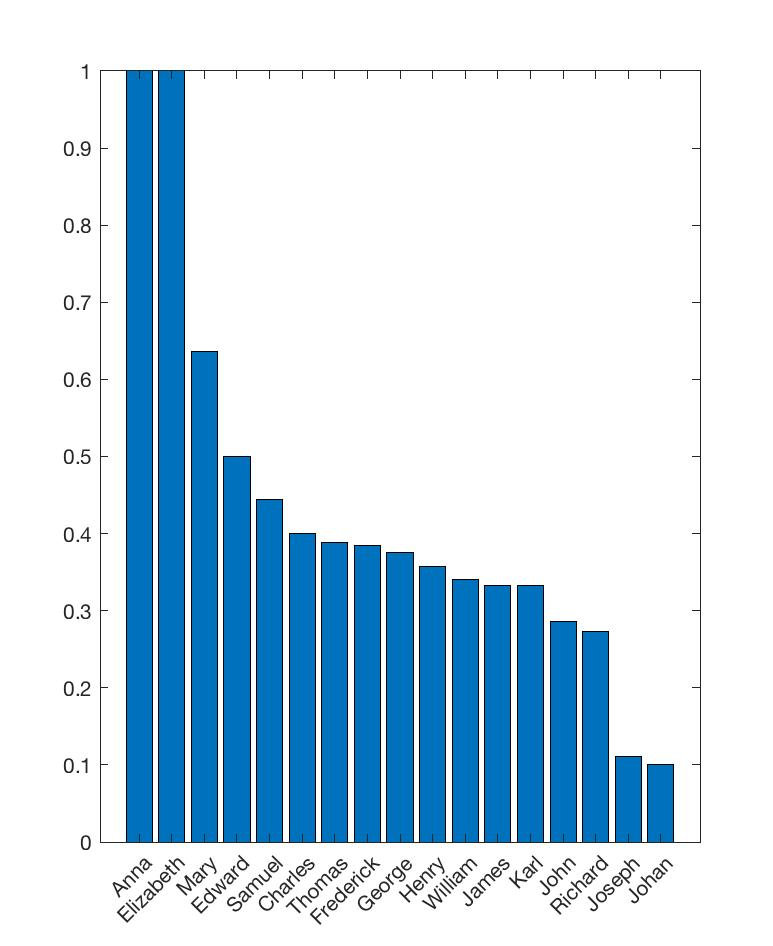
\includegraphics[scale=0.3]{LuckyNames.jpg}
\end{figure}


\end{document}